\begin{figure}[hb]
\centering
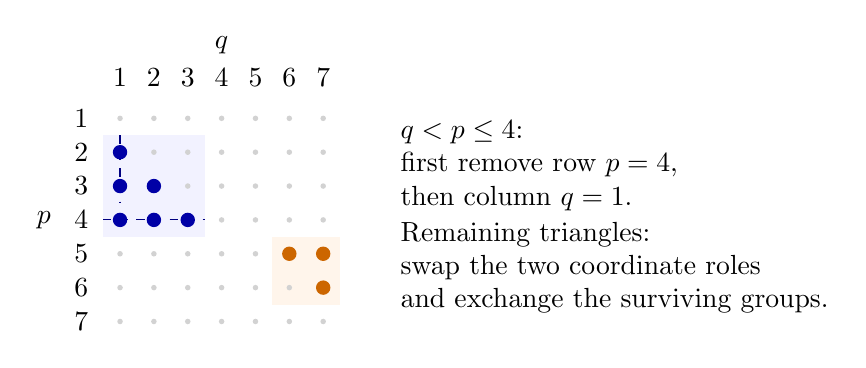
\begin{tikzpicture}[x=.43cm,y=-.43cm]
  \fill[blue!5] (.5,1.5) rectangle (3.5,4.5);
  \fill[orange!8] (5.5,4.5) rectangle (7.5,6.5);
  \draw[blue!50!black,dashed] (.5,4)--(3.5,4);
  \draw[blue!50!black,dashed] (1,1.5)--(1,3.5);
  \foreach \p in {1,...,7}{
    \node[left] at (.35,\p) {$\p$};
    \node[above] at (\p,.35) {$\p$};
    \foreach \q in {1,...,7}{
      \fill[gray!35] (\q,\p) circle (1.0pt);
    }
  }
  \foreach \p/\q in {2/1,3/1,3/2,4/1,4/2,4/3}
    \fill[blue!65!black] (\q,\p) circle (2.6pt);
  \foreach \p/\q in {5/6,5/7,6/7}
    \fill[orange!80!black] (\q,\p) circle (2.6pt);
  \node at (-1.25,4) {$p$};
  \node at (4,-1.15) {$q$};
  \node[anchor=west,align=left] at (9,2.4)
    {$q<p\le4$:\\first remove row $p=4$,\\then column $q=1$.};
  \node[anchor=west,align=left] at (9,5.4)
    {Remaining triangles:\\swap the two coordinate roles\\and exchange the surviving groups.};
\end{tikzpicture}
\caption{The evaluation pattern $Q_s$ for $s=3$, with $n=7$ and $s^2=9$
selected pairs. Removing row $p=s+1$ and then column $q=1$
leaves the pattern for $s-1$ after swapping coordinates and
relabeling the two groups. The gray points are unselected pairs.}
\label{fig:triangular-grid}
\end{figure}
